\chapter{广度优先搜索}
当题目看不出任何规律,既不能用分治,贪心,也不能用动规时,这时候万能方法——搜索,
就派上用场了。搜索分为广搜和深搜,广搜里面又有普通广搜,双向广搜,A*搜索等。
深搜里面又有普通深搜,回溯法等。

广搜和深搜非常类似(除了在扩展节点这部分不一样),二者有相同的框架,如何表示一个状态?
如何扩展节点?如何判重?尤其是判重,解决了这个问题,基本上整个问题就解决了。


\section{走迷宫} %%%%%%%%%%%%%%%%%%%%%%%%%%%%%%


\subsubsection{描述}
一个迷宫由$n$行$m$列的单元格组成,每个单元格要么是空地(用0表示),要
么是障碍物(用1表示)。你的任务是找到一条从入口到出口的最短移动序列,
其中UDLR分别表示上下左右四个方向。任何时候都不能再障碍物格子中,也不
能走到迷宫之外。入口和出口保证是空地。$n,m \leq 100$。

\subsubsection{分析}
既然求的是“最短”,很自然的思路是用BFS。举个例子,在如下图所示的迷宫中,假设
入口是左上角$(0,0)$,我们就从入口开始用BFS遍历迷宫,就可以算出从入口到
所有点的最短路径(如图~\ref{fig:maze}(a)所示),以及这些路径上每个节点的
前驱(如图~\ref{fig:maze}(b)所示)。

\begin{center}
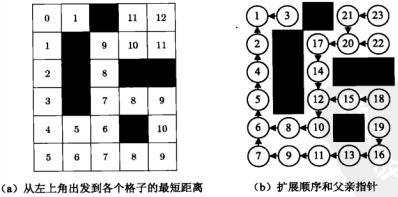
\includegraphics{maze.png}\\
\figcaption{用BFS求迷宫中最短路径}\label{fig:maze}
\end{center}

\subsubsection{代码}
\begin{Codex}[label=maze.c]
#include <stdio.h>
#include <string.h>

#define MAXN 100

// 迷宫的行数,列数
int n, m;
// 迷宫,0表示空地,1表示障碍物
int G[MAXN][MAXN];
// 标记格子是否已访问过
int visited[MAXN][MAXN];
// 每个格子的前驱
int father[MAXN][MAXN];
// 前趋到该格子的前进方向
int last_direction[MAXN][MAXN];

// 四个方向
const char name[4] = {'U','R','D','L'};
const int dx[4] = {-1, 0, 1, 0}; // 行
const int dy[4] = {0, 1, 0, -1}; // 列

// 队列
int q[MAXN * MAXN];

/*
 * @brief 广搜
 *
 * @param[in] x 入口的x坐标
 * @param[in] y 入口的y坐标
 * @return 无
 */
void bfs(int x, int y) {
    int front = 0, rear = 0;
    int u = x * m + y;
    int d; // 方向
    
    father[x][y] = u; // 打印路径时的终止条件
    visited[x][y] = 1;// 千万别忘记了标记此处的访问记录
    q[rear++] = u;
    while (front < rear) {
        u = q[front++];
        x = u / m;    y = u % m;
        for(d = 0; d < 4; d++) { // 代表四个方向
            const int nx = x + dx[d];
            const int ny = y + dy[d];
            
            if (nx >= 0 && nx < n && ny >= 0 && ny < m &&  // //(nx, ny)没有出界
                !G[nx][ny] && !visited[nx][ny]) { // 不是障碍且没被访问过
                const int v = nx * m + ny;
                q[rear++] = v;
                father[nx][ny] = u; // 记录(nx, ny)的前趋
                visited[nx][ny] = 1; // 访问记录
                last_direction[nx][ny] = d; // 记录从(x, y)到(nx, ny)的方向
            }
        }
    }
}

/*
 * @brief 递归实现路径输出
 *
 * 如果格子(x, y)有父亲(fx, fy),需要先打印出从入口到(fx, fy)的最短路径,然后再
 * 打印从 (fx, fy)到 (x,y) 的移动方向。
 *
 * @param[in] x 目标点的x坐标
 * @param[in] y 目标点的y坐标
 * @return 无
 */
void print_path_r(const int x, const int y) {
    const int fx = father[x][y] / m;
    const int fy = father[x][y] % m;
    if (fx != x || fy != y) {
        print_path_r(fx, fy);
        putchar(name[last_direction[x][y]]);
    }
}

int direction[MAXN * MAXN];
/*
 * @brief 显式栈实现路径输出
 *
 * @param[in] x 目标点的x坐标
 * @param[in] y 目标点的y坐标
 * @return 无
 */
void print_path(int x, int y) {
    int c = 0;
    while(1) {
        const int fx = father[x][y] / m;
        const int fy = father[x][y] % m;
        if (fx == x && fy == y) break;
        direction[c++] = last_direction[x][y];
        x = fx;
        y = fy;
    }
    while (c--) {
        putchar(name[direction[c]]);
    }
}

/*
Sample Input
6 5
00100
01000
01011
01000
00010
00000
Sample Output
(0,0)-->(0,4), DDDDRRUUURUR
*/
int main(void) {
    int i, j;
    char s[MAXN];

    scanf("%d%d", &n, &m);

    for(i = 0; i < n; i++) {
        scanf("%s", s);
        for(j = 0; j < m; j++) {
            G[i][j] = s[j] - '0';
        }
    }

    printf("从入口到出口迷宫路径:\n");
    bfs(0, 0);    // (0, 0)是入口
    print_path(0, 4); // (0, 4) 是出口
    printf("\n");
    return 0;
}
\end{Codex}

\subsubsection{相关的题目}
与本题相同的题目:
\begindot
\item 《算法竞赛入门经典》\footnote{刘汝佳,算法竞赛入门经典,清华大学出版社,2009}第108页6.4.2节
\item  POJ 3984 迷宫问题, \myurl{http://poj.org/problem?id=3984}
\myenddot

与本题相似的题目:
\begindot
\item  POJ 2049 Finding Nemo, \myurl{http://poj.org/problem?id=2049}
\myenddot


\section{八数码问题} %%%%%%%%%%%%%%%%%%%%%%%%%%%%%%
\label{subsec:eightDigits}

\subsubsection{描述}
编号为1$\sim$8的8个正方形滑块摆成3行3列,有一个格子空着,如图~\ref{fig:eightDigits}所示。

\begin{center}
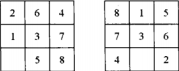
\includegraphics{eight-digits.png}\\
\figcaption{用BFS求迷宫中最短路径}\label{fig:eightDigits}
\end{center}

每次可以把与空格相邻的滑块(有公共边才算相邻)移到空格中,而它原
来的位置就成了新的空格。目标局面固定如下(用$x$表示空格):
\begin{Code}
1 2 3
4 5 6
7 8 x
\end{Code}

给定初始局面,计算出最短的移动路径。

\subsubsection{输入}
用一行表示一个局面,例如下面的这个局面:
\begin{Code}
 1  2  3
 x  4  6
 7  5  8
\end{Code}
可以表示为 1 2 3 x 4 6 7 5 8。 

\subsubsection{输出}
如果有解答,输出一个由四个字母'r','l','u','d'组成的移动路径。
如果没有,输出"unsolvable"。 

\subsubsection{样例输入}
\begin{Code}
2  3  4  1  5  x  7  6  8
\end{Code}

\subsubsection{样例输出}
\begin{Code}
ullddrurdllurdruldr
\end{Code}

\subsubsection{分析}
计算“最短”,很自然的想到BFS。

如何表示一个状态?本题是一个3*3的棋盘,状态有9!个,可以用一个32位整数表示,但15!已经超过32位整数的
范围,21!超过了64位整数的范围,因此4*4的棋盘可以用一个64位整数表示。超过4*4的棋盘,则无法用整数来
表示了,可以用一个数组来表示。

如何判重?用哈希表或者集合。哈希表的话,由于C++ STL 还没有 \fn{std::hashset},
需要自己实现哈希表,然后由于本题的特殊性,存在一种完美哈希(perfect hashing)方案。集合可以直接
使用\fn{std::set}。总结起来,有以下三个方法:
\begindot
\item 把排列变成整数,这是一种完美哈希,即不存在冲突
\item 用普通的哈希表,这种方法通用一些,速度也略慢。手工实现哈希表,把哈希值相同的组成一个单链表,
\item 用 \fn{std::set} 实现判重,代码最短,速度也最慢(本题用这个方法会TLE)。建议把该方法作为“跳板”,
先写一个STL版的程序,确保主算法正确,然后把\fn{std::set}替换成自己写的哈希表。
\myenddot

此题更优的解法还有双向BFS(见\S \ref{sec:biBFS}),A*算法(见\S \ref{sec:astar})。

\subsubsection{代码}
\begin{Codex}[label=eight_digits_bfs.c]
#include <stdio.h>
#include <string.h>
#include <assert.h>

#define DIGITS 9 // 棋盘中数字的个数,也是变进制数需要的位数
#define     MATRIX_EDGE 3       // 棋盘边长

// 3x3的棋盘,状态最多有 9!种
#define     MAX         362880

typedef int state_t[DIGITS]; // 单个状态

state_t q[MAX]; // 队列,也是哈希表
int front, rear;
int distance[MAX - 1]; // 由初始状态到本状态的最短步数
int father[MAX - 1]; // 父状态,初始状态无父状态
char move[MAX - 1]; // 父状态到本状态的移动方向

// 目标状态
const int goal[] = {1, 2, 3, 4, 5, 6, 7, 8, 0};
const int space_number = 0; // 空格对应着数字 0

// 上下左右四个方向
const int dx[] = {-1, 1, 0, 0};
const int dy[] = {0, 0, -1, 1};
const char dc[] = { 'u', 'd', 'l', 'r' };

/**
 * @brief 初始化哈希表.
 * @return 无
 */
void init_lookup_table(); // 版本 1

/**
 * @brief 插入到 visited表中.
 * @param[in] index 状态在队列中的位置
 * @return 成功返回1,失败返回0
 */
int try_to_insert(const int index);

void init_lookup_table_hash(); // 版本2
int try_to_insert_hash(const int index);

void init_lookup_table_stl(); // 版本3
int try_to_insert_stl(const int index);

/**
 * @brief 单向BFS.
 * @return 返回目标状态在队列q中的下标 ,失败则返回0
 */
int bfs() {
    // 三个版本随意切换
    init_lookup_table();
    // init_lookup_table_hash();
    // init_lookup_table_stl(); // 这个版本会 Time Limit Exceeded

    while (front < rear) {
        int x, y, z, d;
        const state_t*s = &(q[front]);
        if (memcmp(goal, *s,sizeof(state_t)) == 0) {
            return front;  // 找到目标状态,成功返回
        }
        for (z = 0; z < DIGITS; z++)  if ((*s)[z] == space_number) {
            break;  // 找 0 的位置
        }
        
        x=z / MATRIX_EDGE, y=z % MATRIX_EDGE; // 获取行列编号
        for (d=0; d < 4; d++) {  // 向四个方向扩展
            const int newx = x + dx[d];
            const int newy = y + dy[d];
            const int newz = newx * MATRIX_EDGE + newy;

            if (newx >= 0 && newx < MATRIX_EDGE && newy >= 0 &&
                newy < MATRIX_EDGE) { // 没有越界
                state_t *t = &(q[rear]);
                memcpy(t, s, sizeof((*s)));
                assert((*s)[z] == space_number);
                (*t)[newz] = space_number;
                (*t)[z] = (*s)[newz];

                // 三个版本随意切换
                if (try_to_insert(rear)) { // 利用查找表判重
                // if (try_to_insert_hash(rear)) {
                // if (try_to_insert_stl(rear)) {
                    father[rear] = front;
                    move[rear] = dc[d];
                    distance[rear] = distance[front] + 1;
                    rear++;
                } 
            }
        }

        front++;
    }

    return 0;//失败 
}


/**
 * @brief 输入.
 * @return 无
 */
void input() {
    int ch, i;
    for (i = 0; i < DIGITS; ++i) {
        do {
            ch = getchar();
        } while ((ch != EOF) && ((ch < '1') || (ch > '8')) && (ch != 'x'));
        if (ch == EOF) return;
        if (ch == 'x') q[0][i] = 0; // x 映射成数字 0
        else           q[0][i] = ch - '0';
    }
    front = 0; rear = 1;
    father[0] = 0; // 初始状态无父状态
    distance[0] = 0;
    move[0] = -1;
    return;
}

int top = -1;
char stack[MAX];
/**
 * @brief 打印从初始状态到目标状态的移动序列.
 * @param[in] index 目标状态在队列q中的下标
 * @return 无
 */
void output(const int index) {
    int i;
    for (i = index; i > 0; i = father[i]) {
        stack[++top] = move[i];
    }
    for (i = top; i >= 0; --i) {
        printf("%c", stack[i]);
    }
    printf("\n");
}

int main() {
    int ans;

    input();
    
    ans = bfs();
    if ( ans > 0) {
        output(ans);
    } else {
        printf("no solution\n");
    }
    return 0;
}

/***********************方案1 把排列变成整数**************************/
// 9 位变进制数(空格)能表示0到(9!-1)内的所有自然数,恰好有9!个,
// 与状态一一对应,因此可以把状态一一映射到一个9位变进制数

// 9 位变进制数,每个位数的单位,0!~8!
const int fac[] = {40320, 5040, 720, 120, 24, 6, 2, 1, 1};

// 采用本方案,由于是完美哈希,没有冲突,
// 可以用 MAX 代替 MAX_HASH_SIZE,减少内存占用量
int visited[MAX]; // 历史记录表

/** 初始化哈希表. */
void init_lookup_table() {
    memset(visited, 0, sizeof(visited));
}

/**
 * @brief 计算状态的hash值,这里用康托展开,是完美哈希.
 *
 * @param[in] s 状态
 * @return 序数,作为hash值
 */
int hash(const state_t *s) {
    int i, j;
    int key = 0; // 将 q[index] 映射到整数 key
    for (i = 0; i < 9; i++) {
        int cnt = 0;
        for (j = i + 1; j < 9; j++) if ((*s)[i] > (*s)[j]) cnt++;
        key += fac[i] * cnt;
    }
    return key;
}

/**
 * @brief 插入到 visited表中.
 * @param[in] index 状态在队列中的位置
 * @return 成功返回1,失败返回0
 */
int try_to_insert(const int index) {
    const int key = hash(&q[index]); // 将 q[index] 映射到整数 code
    
    if (visited[key]) return 0;
    else visited[key] = 1;

    return 1;
}

/**************************方案2 哈希表**********************************/
#define MAX_HASH_SIZE  1000000  // 状态的哈希表容量,比 9! 大即可

int head[MAX_HASH_SIZE];
int next[MAX];

void init_lookup_table_hash() {
    memset(head, 0, sizeof(head));
    memset(next, 0, sizeof(next));
}
int hash2(const state_t *s) {
    int i;
    int v = 0;
    for(i = 0; i < 9; i++) v = v * 10 + (*s)[i];
    return v % MAX_HASH_SIZE;
}

int try_to_insert_hash(const int index) {
    const int h = hash2(&(q[index]));
    int u = head[h]; // 从表头开始查找单链表
    while(u) {
        // 找到了,插入失败
        if(memcmp(q[u], q[index], sizeof(state_t)) == 0) return 0;
        u = next[u]; // 顺着链表继续找
    }
    next[index] = head[h]; // 插入到链表中
    head[h] = index; // head[h]和 next[index] 组成了一个节点
    return 1;
}

/****************************方案3 STL************************************/
#include <set>
struct cmp {
    bool operator() (int a, int b) const {
        return memcmp(&q[a], &q[b], sizeof(state_t)) < 0;
    }
};
std::set<int, cmp> visited_set;

void init_lookup_table_stl() { visited_set.clear(); }

int try_to_insert_stl(const int index) {
    if (visited_set.count(index)) return 0;
    visited_set.insert(index);
    return 1;
}
\end{Codex}

\subsubsection{相关的题目}
与本题相同的题目:
\begindot
\item 《算法竞赛入门经典》\footnote{刘汝佳,算法竞赛入门经典,清华大学出版社,2009} 第131页7.5.3节
\item  POJ 1077 Eight, \myurl{http://poj.org/problem?id=1077}
\myenddot

与本题相似的题目:
\begindot
\item  POJ 2893 M × N Puzzle, \myurl{http://poj.org/problem?id=2893}
\myenddot


\section{四子连棋} %%%%%%%%%%%%%%%%%%%%%%%%%%%%%%

\subsubsection{描述}
在一个4*4的棋盘上摆放了14颗棋子,其中有7颗白色棋子,7颗黑色棋子,有两个空白地带,任何一颗黑白
棋子都可以向上下左右四个方向移动到相邻的空格,这叫行棋一步,黑白双方交替走棋,任意一方可以先走,
如果某个时刻使得任意一种颜色的棋子形成四个一线(包括斜线),这样的状态为目标棋局。

\subsubsection{输入}
一个4*4的初始棋局,黑棋子用B表示,白棋子用W表示,空格地带用O表示。

\subsubsection{输出}
移动到目标棋局的最少步数。

\subsubsection{样例输入}
\begin{Code}
BWBO
WBWB
BWBW
WBWO
\end{Code}

\subsubsection{样例输出}
\begin{Code}
5
\end{Code}

\subsubsection{分析}
求最少步数,很自然的想到广搜。

如何表示一个状态?用一个二维数组\fn{int board[4][4]}表示,还需要记录该状态是由白子还是黑子移动而导致的,走到该状态已经花费的步数。

如何扩展节点?每一步,从队列弹出一个状态,两个空格都可以向四个方向扩展,把得到的状态入队列。

如何判重?棋盘用二维矩阵存储,用0表示空格,1表示黑色,2表示白色,所以最后可以看成一个16位的三进制数。
用这个数作为棋盘的编码,就可以用来判重了。注意,本题要黑白交替走,所以我们要区分状态是由白子还是黑子移动而导致的。

可以用C++的\fn{std::map}来判重,
\begin{Code}
/* history[0]记录白子的历史,history[1]记录黑子的历史. */
std::map<int, bool> history[2];
\end{Code}

也可以开一个大数组当做哈希表,
\begin{Code}
#define HASH_MOD 43036875 /* hash表大小 */
/* history[0]记录白子的历史,history[1]记录黑子的历史. */
bool history[2][HASH_MOD];
\end{Code}

\subsubsection{代码}
\begin{Codex}[label=four_adjacent.c]
/** wikioi 1004 四子连棋  , http://www.wikioi.com/problem/1004 */
#include <stdio.h>
#include <stdlib.h>
#include <memory.h>
#include <stdbool.h>

#define LEN 4   /* 边长 */
#define RADIX 3 /* 三进制 */
#define HASH_MOD 43036875 /* hash表大小 */

/* 右,左,上,下(左下角为坐标原点)*/
const int dx[] = { 1, -1, 0, 0 };
const int dy[] = { 0, 0, 1, -1 };

/** 状态. */
typedef struct status_t {
    int hash; /* board 对应的hash值  */
    int step; /* 走了步到达本状态 */
    int last; /* 本状态是由白子还是黑子移动而导致的 */
    int board[LEN][LEN]; /* 棋局,1表示黑子,2表示白子,0表示空白 */
} status_t;

status_t first; /* 初始输入的棋局. */

/* history[0]记录白子的历史,history[1]记录黑子的历史. */
bool history[2][HASH_MOD];


typedef status_t queue_elem_t; /* 元素的类型 */

/* 等价于复制粘贴,这里为了节约篇幅,使用include,在OJ上提交时请用复制粘贴 */
#include "queue.c"

/** 队列 */
queue_t q;


/**
 * @brief 计算棋盘所表示的三进制数转化为十进制数.
 * 棋盘用二维矩阵存储,用0表示空格,1表示黑色,2表示白色,所以最后可以看成
 * 一个16位的三进制数。最大为
 * 2222
 * 2221
 * 1111
 * 1100
 * 值为 43036875。
 * @return 棋盘所表示的三进制数转化为十进制数
 */
//TODO:共C16 7×C9 2个状态,用类似康托的方法储存
int hash(const int board[LEN][LEN]) {
    int i, j;
    int ret = 0;
    for (i = 0; i < LEN; i++) {
        for (j = 0; j < LEN; j++) {
            ret = ret * RADIX + board[i][j];
        }
    }
    return ret;
}

/**
 * 检查是否有四个棋子连成一线.
 * @return 有,返回1,没有,返回0
 */
bool check(status_t a) {
    int i, j;
    for (i = 0; i < LEN; i++) {  /* 逐行检查 */
        int flag = 1;  /* 某一行全是同一颜色 */
        for (j = 1; j < LEN; j++)
            if (a.board[i][j - 1] != a.board[i][j])
                flag = 0;
        if (flag)
            return 1;
    }
    for (j = 0; j < LEN; j++) { //逐列检查
        int flag = 1;  /* 某一行全是同一颜色 */
        for (i = 1; i < LEN; i++)
            if (a.board[i][j] != a.board[i - 1][j])
                flag = 0;
        if (flag)
            return 1;
    }
    /* 斜线 */
    if (a.board[0][0] == a.board[1][1] && a.board[1][1] == a.board[2][2]
            && a.board[2][2] == a.board[3][3])
        return 1;
    if (a.board[0][3] == a.board[1][2] && a.board[1][2] == a.board[2][1]
            && a.board[2][1] == a.board[3][0])
        return 1;
    return 0;
}

/** (x,y)是空白棋子的位置,将(x,y)朝(dx[k],dy[k])方向移动. */
void move(status_t now, int x, int y, int k) {
    status_t next = now;
    int nextx = x + dx[k];
    int nexty = y + dy[k];

    /* 越界 */
    if (nextx < 0 || nextx >= LEN)
        return;
    if (nexty < 0 || nexty >= LEN)
        return;

    if (next.board[nextx][nexty] == next.last)
        return; /* 必须黑白交替走 */

    next.last = 3 - next.last;
    /* swap */
    {
        int temp = next.board[x][y];
        next.board[x][y] = next.board[nextx][nexty];
        next.board[nextx][nexty] = temp;
    }
    next.hash = hash(next.board);
    next.step++;
    if (check(next)) {
        printf("%d\n", next.step);
        exit(0);
    }
    if (!history[next.last - 1][next.hash]) {
        history[next.last - 1][next.hash] = true;
        queue_push(&q, next);
    }
}

void bfs() {
    int i, j, k;
    first.hash = hash(first.board);
    first.last = 1;
    queue_push(&q, first);
    first.last = 2;
    queue_push(&q, first);

    while (!queue_empty(&q)) {
        status_t now = queue_front(&q);
        queue_pop(&q);
        int x1 = -1, x2 = -1, y1 = -1, y2 = -1; //两个空白的格子
        for (i = 0; i < LEN; i++) {
            for (j = 0; j < LEN; j++) {
                if (now.board[i][j] == 0) {
                    if (x1 == -1 && y1 == -1) {
                        x1 = i;
                        y1 = j;
                    } else {
                        x2 = i;
                        y2 = j;
                    }
                }
            }
        }
        for (k = 0; k < 4; k++) {
            move(now, x1, y1, k);
            move(now, x2, y2, k);
        }
    }
}

int main() {
    int i, j;
    char s[LEN + 1];
    queue_init(&q, 32);
    for (i = 0; i < LEN; i++) {
        scanf("%s", s);
        for (j = 0; j < LEN; j++) {
            if (s[j] == 'B')
                first.board[i][j] = 1;
            else if (s[j] == 'W')
                first.board[i][j] = 2;
        }
    }
    bfs();
    queue_uninit(&q);
    return 0;
}
\end{Codex}

\subsubsection{相关的题目}
与本题相同的题目:
\begindot
\item  wikioi 1004 四子连棋, \myurl{http://www.wikioi.com/problem/1004/}
\myenddot

与本题相似的题目:
\begindot
\item  None
\myenddot


\section{双向BFS} %%%%%%%%%%%%%%%%%%%%%%%%%%%%%%
\label{sec:biBFS}


\subsection{八数码问题}
题目见 \S \ref{subsec:eightDigits}。

\subsubsection{代码}

\begin{Codex}[label=eight_digits_bibfs.c]

\end{Codex}


\section{A*算法} %%%%%%%%%%%%%%%%%%%%%%%%%%%%%%
\label{sec:astar}


\subsection{八数码问题}
题目见 \S \ref{subsec:eightDigits}。

\subsubsection{代码}
\begin{Codex}[label=eight_digits_astar.c]
/**
 简单解释几个要点,便于理解代码.
 1. 怎么判断是否有解?只要计算出的逆序个数总和为奇数,该数据必然无解
 2. 如何判断某一状态是否到过?本题存在一种完美哈希方案,即用康托展开。
    详见 http://128kj.iteye.com/blog/1699795
    2.1.将一个状态视为数字 0-8 的一个排列,将此排列转化为序数,作为此状
 态的 HASH 值。0表示空格.转化算法此处不再赘述。

    2.2.排列转化为序数,用序数作为hash值
    例,1 2 3 这三个数字的全排列,按字典序,依次为
 123 -- 0
 132 -- 1
 213 -- 2
 231 -- 3
 312 -- 4
 321 -- 5
 其中,左侧为排列,右侧为其序数。
 
 3.使用数据结构 堆 加速挑选最优值。
 
 4.函数 g 的计算,此状态在搜索树中已经走过的路径的节点数.
 
 5.估价函数 h ,采用曼哈顿距离, 见代码 calcH 函数。曼哈顿距离的定义是,
 假设有两个点(x1,y1),(x2,y2),则曼哈顿距离L1=|x1-x2| + |y1-y2|
 */
#include <stdio.h>
#include <string.h>
#include <stdlib.h>

// 3x3的棋盘,状态最多有 9!种
// 8位变进制数(空格)能表示0到(9!-1)内的所有自然数,恰好有9!个,
// 与状态一一对应,因此可以把状态一一映射到一个8位变进制数
#define     MAX         362880

#define DIGITS 9 // 棋盘中数字的个数,也是变进制数需要的位数
#define     MATRIX_EDGE 3       // 棋盘边长

#define     MOD         10      // 按十取模

typedef struct {
    int state; // 状态
    int parent;     // 父状态
    int flag;   // -1 表示已经展开过了closed,0表示死节点,1 表示还未展开, open
    int g, h, f; // 三个评估函数
    char choice;  // 左右上下四个方向移动,见全局常量 DI DJ DC
} state_t;

state_t states[MAX];  // 全局的一条状态变化路径

int  startIndex, goalIndex; // 开始状态,目标状态对应的hash值

// 目标状态
const int goal = 123456780;
// 每个数字在棋盘中的位置,例如0,在(1,1)=4这个位置上
const int goal_pos[DIGITS] = {8,0,1,2,3,4,5,6,7};
const int space_number = 0; // 空格对应着数字 0

// 上下左右四个方向
const int DI[] = {-1, 1, 0, 0};
const int DJ[] = {0, 0, -1, 1};
const char DC[] = { 'u', 'd', 'l', 'r' };

// 9 位变进制数,每个位数的单位,0!~8!
const int fac[] = {40320, 5040, 720, 120, 24, 6, 2, 1, 1};

/**
 * @brief 计算状态的hash值,这里用康托展开,是完美哈希.
 *
 * @param[in] s 当前状态
 * @return 序数,作为hash值
 */
int hash(int s) {
    int i, j;
    int d[DIGITS];
    int key = 0;

    for(i = DIGITS - 1; i >=0; i--) {
        d[i] = s % MOD;
        s /= MOD;
    }
    
    for (i = 0; i < DIGITS; i++) {
        int c = 0; // 逆序数
        for (j = i + 1; j < DIGITS; j++) {
            if(d[j] < d[i]) {
                c++;
            }
        }
        key += c * fac[i];
    }
    
    return key;
}


/**
 * 估价函数h。
 * @param s 状态
 * @return 预估代价
 */
int calcH(int s) {
    int i;
    int h = 0;
    
    for (i = DIGITS - 1; i >= 0; --i) {
        const int p = s % 10;
        s /= 10;
        // 曼哈顿距离
        h += abs(i / MATRIX_EDGE - goal_pos[p] / MATRIX_EDGE) +
            abs(i % MATRIX_EDGE - goal_pos[p] % MATRIX_EDGE);
    }
    return h;
}

/**
 * @brief 输入.
 * @return  成功返回数字,失败返回0
 * @remark 《算法竞赛入门经典》第131页7.5.3节,是用0表示空格,
 * POJ 1077是用'x'表示空格,前者简化了一点,POJ 1077还需要把'x'映射成0
 */
int input() {
    int ch, i;
    int start = 0;
    for (i = 0; i < DIGITS; ++i) {
        do {
            ch = getchar();
        } while ((ch != EOF) && ((ch < '1') || (ch > '8')) && (ch != 'x'));
        if (ch == EOF) return 0;
        if (ch == 'x') start = start * MOD + space_number; // x 映射成数字 0
        else             start = start * MOD + ch - '0';
    }
    return start;
}

/**
 * 计算一个排列的逆序数,0 除外.
 */
int inversion_count(int permutation) {
    int i, j;
    int d[DIGITS];
    int c = 0; // 逆序数

    for(i = DIGITS - 1; i >=0; i--) {
        d[i] = permutation % MOD;
        permutation /= MOD;
    }
    
    for (i = 1; i < DIGITS; i++)  if (d[i] != space_number) {
        for (j = 0; j < i; j++) {
            if(d[j] != space_number) {
                if (d[j] > d[i]) {
                    c++;
                }
            }
        }
    }
    return c;
}

/**
 * 判断是否无解.
 *
 * 求出除0之外所有数字的逆序数之和,也就是每个数字后面比它小的数字的个数的和,
 * 称为这个状态的逆序。若两个状态的逆序奇偶性相同,则可相互到达,否则不可相互到达。
 * 由于原始状态的逆序数为0(偶数),因此逆序数为偶数的目标状态有解。
 *
 * @param s 目标状态
 * @return 1表示无解,0表示有解
 */
int not_solvable(const int s) {
    return inversion_count(s) % 2;
}

// 存放 next()的输出结果
char choice[4]; // 四个防线
int nextIndex[4]; // 接下来的四个状态

/*
 * @brief 向四个方向扩展
 * @param[in] s 状态
 * @return 无
 */
void next(int s) {
    int i, j, k;
    int p[MATRIX_EDGE][MATRIX_EDGE]; // 一个状态对应的矩阵
    int i0, j0;  // 空格位置

    for (i = MATRIX_EDGE - 1; i >= 0; i--) {
        for (j = MATRIX_EDGE - 1; j >= 0; j--) {
            p[i][j] = s % MOD;
            s /= MOD;
            if (p[i][j] == space_number) {
                i0 = i;
                j0 = j;
            }
        }
    }
    // 向四个方向探索
    for (k = 0; k < 4; ++k) {
        const int sx = i0 + DI[k]; // 空格的新位置(sx, sy)
        const int sy = j0 + DJ[k];
        if ((sx >= 0) && (sx < 3) && (sy >= 0) && (sy < 3)) {
            int key;
            p[i0][j0] = p[sx][sy];
            p[sx][sy] = space_number;
            // 移动空格后,计算新的状态
            s = 0;
            for (i = 0; i < MATRIX_EDGE; i++)
                for (j = 0; j < MATRIX_EDGE; j++)
                    s = s * MOD + p[i][j];
            p[sx][sy] = p[i0][j0]; // 将矩阵还原,(i0, j0)可以不管
            
            key = nextIndex[k] = hash(s);
            choice[k] = DC[k];
            if (states[key].state == 0) { // 该状态还没有出现过
                states[key].state = s;
                states[key].h = calcH(s);
            }
        } else {// 越界了
            nextIndex[k] = -1;
        }
    }
}

/* 等价于复制粘贴,这里为了节约篇幅,使用include,在OJ上提交时请用复制粘贴 */
#include "heap.c"
heap_t heap;
int heapIndex[MAX + 4]; // 状态 x 在heap中的下标

/**
 * @brief A*搜索
 * @param[in] start 初始状态
 * @return 如果无解,返回0,如果有解返回1
 */
int astar(const int start) {
    int i, j, k, ng, nf;
    if (not_solvable(start)) return 0;

    startIndex = hash(start);
    goalIndex  = hash(goal);
    if (start == goal) return 1;
    
    memset(states, 0, sizeof(states));
    states[startIndex].state = start;
    states[startIndex].flag    = 1;
    states[startIndex].g       = 0;
    states[startIndex].h       = states[startIndex].f = calcH(start);

    heap_push(&heap, startIndex);
    while(!heap_empty(&heap)) {
        i = heap_top(&heap); heap_pop(&heap);
        if (i == goalIndex) return 1; // 找到目标,返回

        states[i].flag = -1;
        ng = states[i].g + 1;
        next(states[i].state);
        for (k = 0; k < 4; ++k) {
            j = nextIndex[k];
            if (j < 0) continue;
            nf = ng + states[j].h;
            if ((states[j].flag == 0) || ((states[j].flag == 1) &&
                (nf < states[j].f))) {
                states[j].parent = i;
                states[j].choice = choice[k];
                states[j].g    = ng;
                states[j].f    = nf;
                if (states[j].flag > 0) {
                    heap_sift_up(&heap, heapIndex[j]);
                    heap_sift_down(&heap, heapIndex[j]);
                } else {
                    heap_push(&heap, j);
                    states[j].flag = 1;
                }
            }
        }
    }
    return 0;
}

/* 等价于复制粘贴,这里为了节约篇幅,使用include,在OJ上提交时请用复制粘贴 */
#include "stack.c"
/**
 * @brief 打印移动序列.
 * @return 无
 */
void output() {
    int i;
    stack_t stack;
    stack_init(&stack, MAX);

    for (i = goalIndex; i != startIndex; i = states[i].parent) {
        stack_push(&stack, states[i].choice);
    }
    while(!stack_empty(&stack)) {
        printf("%c", stack_top(&stack));
        stack_pop(&stack);
    }
    
    printf("\n");
    stack_uninit(&stack);
}

/**
 * @brief 打印棋盘的每次变化.
 * @return 无
 */
void output1() {
    int i;
    int d[DIGITS];
    stack_t stack;
    stack_init(&stack, MAX);
    
    for (i = goalIndex; i != startIndex; i = states[i].parent) {
        stack_push(&stack, states[i].state);
    }
    stack_push(&stack, states[startIndex].state);
    
    while(!stack_empty(&stack)) {
        stack_elem_t tmp = stack_top(&stack); 
        stack_pop(&stack);
        for(i = DIGITS - 1; i >=0; i--) {
            d[i] = tmp % MOD;
            tmp /= MOD;
        }
        for(i = 0; i < DIGITS; i++) {
            if((i + 1) % MATRIX_EDGE == 0) {
                printf("%d\n", d[i]);
            } else {
                printf("%d ", d[i]);
            }
        }
        printf("\n");
    }
    stack_uninit(&stack);
}

int main() {
    const int start = input();
    heap_init(&heap, MAX + 4, cmp_int);
    if (start > 0) {
        if (astar(start)) {
            output();
        } else {
            printf("no solution\n");
        }
    }
    heap_uninit(&heap);
    return 0;
}
\end{Codex}
